\documentclass[twoside]{book}

% Packages required by doxygen
\usepackage{fixltx2e}
\usepackage{calc}
\usepackage{doxygen}
\usepackage[export]{adjustbox} % also loads graphicx
\usepackage{graphicx}
\usepackage[utf8]{inputenc}
\usepackage{makeidx}
\usepackage{multicol}
\usepackage{multirow}
\PassOptionsToPackage{warn}{textcomp}
\usepackage{textcomp}
\usepackage[nointegrals]{wasysym}
\usepackage[table]{xcolor}

% Font selection
\usepackage[T1]{fontenc}
\usepackage[scaled=.90]{helvet}
\usepackage{courier}
\usepackage{amssymb}
\usepackage{sectsty}
\renewcommand{\familydefault}{\sfdefault}
\allsectionsfont{%
  \fontseries{bc}\selectfont%
  \color{darkgray}%
}
\renewcommand{\DoxyLabelFont}{%
  \fontseries{bc}\selectfont%
  \color{darkgray}%
}
\newcommand{\+}{\discretionary{\mbox{\scriptsize$\hookleftarrow$}}{}{}}

% Page & text layout
\usepackage{geometry}
\geometry{%
  a4paper,%
  top=2.5cm,%
  bottom=2.5cm,%
  left=2.5cm,%
  right=2.5cm%
}
\tolerance=750
\hfuzz=15pt
\hbadness=750
\setlength{\emergencystretch}{15pt}
\setlength{\parindent}{0cm}
\setlength{\parskip}{3ex plus 2ex minus 2ex}
\makeatletter
\renewcommand{\paragraph}{%
  \@startsection{paragraph}{4}{0ex}{-1.0ex}{1.0ex}{%
    \normalfont\normalsize\bfseries\SS@parafont%
  }%
}
\renewcommand{\subparagraph}{%
  \@startsection{subparagraph}{5}{0ex}{-1.0ex}{1.0ex}{%
    \normalfont\normalsize\bfseries\SS@subparafont%
  }%
}
\makeatother

% Headers & footers
\usepackage{fancyhdr}
\pagestyle{fancyplain}
\fancyhead[LE]{\fancyplain{}{\bfseries\thepage}}
\fancyhead[CE]{\fancyplain{}{}}
\fancyhead[RE]{\fancyplain{}{\bfseries\leftmark}}
\fancyhead[LO]{\fancyplain{}{\bfseries\rightmark}}
\fancyhead[CO]{\fancyplain{}{}}
\fancyhead[RO]{\fancyplain{}{\bfseries\thepage}}
\fancyfoot[LE]{\fancyplain{}{}}
\fancyfoot[CE]{\fancyplain{}{}}
\fancyfoot[RE]{\fancyplain{}{\bfseries\scriptsize Generated by Doxygen }}
\fancyfoot[LO]{\fancyplain{}{\bfseries\scriptsize Generated by Doxygen }}
\fancyfoot[CO]{\fancyplain{}{}}
\fancyfoot[RO]{\fancyplain{}{}}
\renewcommand{\footrulewidth}{0.4pt}
\renewcommand{\chaptermark}[1]{%
  \markboth{#1}{}%
}
\renewcommand{\sectionmark}[1]{%
  \markright{\thesection\ #1}%
}

% Indices & bibliography
\usepackage{natbib}
\usepackage[titles]{tocloft}
\setcounter{tocdepth}{3}
\setcounter{secnumdepth}{5}
\makeindex

% Hyperlinks (required, but should be loaded last)
\usepackage{ifpdf}
\ifpdf
  \usepackage[pdftex,pagebackref=true]{hyperref}
\else
  \usepackage[ps2pdf,pagebackref=true]{hyperref}
\fi
\hypersetup{%
  colorlinks=true,%
  linkcolor=blue,%
  citecolor=blue,%
  unicode%
}

% Custom commands
\newcommand{\clearemptydoublepage}{%
  \newpage{\pagestyle{empty}\cleardoublepage}%
}

\usepackage{caption}
\captionsetup{labelsep=space,justification=centering,font={bf},singlelinecheck=off,skip=4pt,position=top}

%===== C O N T E N T S =====

\begin{document}

% Titlepage & ToC
\hypersetup{pageanchor=false,
             bookmarksnumbered=true,
             pdfencoding=unicode
            }
\pagenumbering{roman}
\begin{titlepage}
\vspace*{7cm}
\begin{center}%
{\Large My Project }\\
\vspace*{1cm}
{\large Generated by Doxygen 1.8.11}\\
\end{center}
\end{titlepage}
\clearemptydoublepage
\tableofcontents
\clearemptydoublepage
\pagenumbering{arabic}
\hypersetup{pageanchor=true}

%--- Begin generated contents ---
\chapter{File Index}
\section{File List}
Here is a list of all files with brief descriptions\+:\begin{DoxyCompactList}
\item\contentsline{section}{src/\hyperlink{position__server_8cpp}{position\+\_\+server.\+cpp} }{\pageref{position__server_8cpp}}{}
\item\contentsline{section}{src/\hyperlink{robot__controller_8cpp}{robot\+\_\+controller.\+cpp} }{\pageref{robot__controller_8cpp}}{}
\end{DoxyCompactList}

\chapter{File Documentation}
\hypertarget{position__server_8cpp}{}\section{src/position\+\_\+server.cpp File Reference}
\label{position__server_8cpp}\index{src/position\+\_\+server.\+cpp@{src/position\+\_\+server.\+cpp}}
{\ttfamily \#include \char`\"{}ros/ros.\+h\char`\"{}}\\*
{\ttfamily \#include \char`\"{}my\+\_\+assignment\+\_\+1/\+Target\+\_\+\+Position.\+h\char`\"{}}\\*
Include dependency graph for position\+\_\+server.\+cpp\+:\nopagebreak
\begin{figure}[H]
\begin{center}
\leavevmode
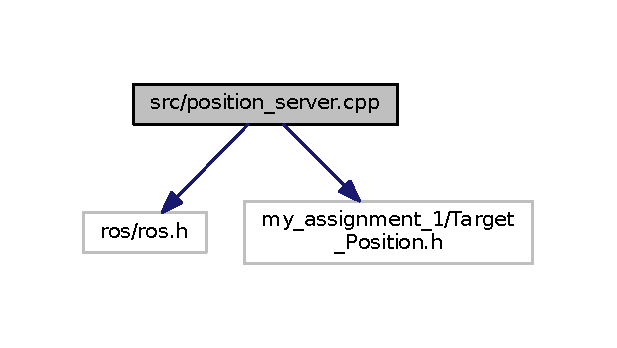
\includegraphics[width=296pt]{position__server_8cpp__incl}
\end{center}
\end{figure}
\subsection*{Macros}
\begin{DoxyCompactItemize}
\item 
\#define \hyperlink{position__server_8cpp_a3f06f0e9f7beb8214afeea0b18ef8377}{min}~-\/6.\+0
\item 
\#define \hyperlink{position__server_8cpp_a2e1da8593b0244d8e9e3b84ef7b35e73}{max}~+6.\+0
\end{DoxyCompactItemize}
\subsection*{Functions}
\begin{DoxyCompactItemize}
\item 
bool \hyperlink{position__server_8cpp_a8b8775a486a432617442ad99d66bd482}{target\+\_\+pos} (my\+\_\+assignment\+\_\+1\+::\+Target\+\_\+\+Position\+::\+Request \&req, my\+\_\+assignment\+\_\+1\+::\+Target\+\_\+\+Position\+::\+Response \&res)
\item 
int \hyperlink{position__server_8cpp_a3c04138a5bfe5d72780bb7e82a18e627}{main} (int argc, char $\ast$$\ast$argv)
\end{DoxyCompactItemize}


\subsection{Macro Definition Documentation}
\index{position\+\_\+server.\+cpp@{position\+\_\+server.\+cpp}!max@{max}}
\index{max@{max}!position\+\_\+server.\+cpp@{position\+\_\+server.\+cpp}}
\subsubsection[{\texorpdfstring{max}{max}}]{\setlength{\rightskip}{0pt plus 5cm}\#define max~+6.\+0}\hypertarget{position__server_8cpp_a2e1da8593b0244d8e9e3b84ef7b35e73}{}\label{position__server_8cpp_a2e1da8593b0244d8e9e3b84ef7b35e73}
\index{position\+\_\+server.\+cpp@{position\+\_\+server.\+cpp}!min@{min}}
\index{min@{min}!position\+\_\+server.\+cpp@{position\+\_\+server.\+cpp}}
\subsubsection[{\texorpdfstring{min}{min}}]{\setlength{\rightskip}{0pt plus 5cm}\#define min~-\/6.\+0}\hypertarget{position__server_8cpp_a3f06f0e9f7beb8214afeea0b18ef8377}{}\label{position__server_8cpp_a3f06f0e9f7beb8214afeea0b18ef8377}
Define constants to fix the limits of the domain 

\subsection{Function Documentation}
\index{position\+\_\+server.\+cpp@{position\+\_\+server.\+cpp}!main@{main}}
\index{main@{main}!position\+\_\+server.\+cpp@{position\+\_\+server.\+cpp}}
\subsubsection[{\texorpdfstring{main(int argc, char $\ast$$\ast$argv)}{main(int argc, char **argv)}}]{\setlength{\rightskip}{0pt plus 5cm}int main (
\begin{DoxyParamCaption}
\item[{int}]{argc, }
\item[{char $\ast$$\ast$}]{argv}
\end{DoxyParamCaption}
)}\hypertarget{position__server_8cpp_a3c04138a5bfe5d72780bb7e82a18e627}{}\label{position__server_8cpp_a3c04138a5bfe5d72780bb7e82a18e627}
/\+Main function\+:

/\+Parameters\+:

int argc, char $\ast$$\ast$argv are mandatory for cpp files

/\+Comments about the code\+:

ros\+::init--$>$initialisation of the node position\+\_\+server

ros\+::\+Node\+Handle n --$>$ set-\/up node\+Handle

ros\+::\+Service\+Server service= n.\+advertise\+Service(\char`\"{}robot/target\+\_\+pos\char`\"{},target\+\_\+pos) --$>$ define server and specify function call\+Back

ros\+::spin()--$>$ blocks the main thread from exiting until R\+OS invokes a shutdown (for example Ctrl+C) \index{position\+\_\+server.\+cpp@{position\+\_\+server.\+cpp}!target\+\_\+pos@{target\+\_\+pos}}
\index{target\+\_\+pos@{target\+\_\+pos}!position\+\_\+server.\+cpp@{position\+\_\+server.\+cpp}}
\subsubsection[{\texorpdfstring{target\+\_\+pos(my\+\_\+assignment\+\_\+1\+::\+Target\+\_\+\+Position\+::\+Request \&req, my\+\_\+assignment\+\_\+1\+::\+Target\+\_\+\+Position\+::\+Response \&res)}{target_pos(my_assignment_1::Target_Position::Request &req, my_assignment_1::Target_Position::Response &res)}}]{\setlength{\rightskip}{0pt plus 5cm}bool target\+\_\+pos (
\begin{DoxyParamCaption}
\item[{my\+\_\+assignment\+\_\+1\+::\+Target\+\_\+\+Position\+::\+Request \&}]{req, }
\item[{my\+\_\+assignment\+\_\+1\+::\+Target\+\_\+\+Position\+::\+Response \&}]{res}
\end{DoxyParamCaption}
)}\hypertarget{position__server_8cpp_a8b8775a486a432617442ad99d66bd482}{}\label{position__server_8cpp_a8b8775a486a432617442ad99d66bd482}
/\+Function call\+Back executed when client calls

/\+Parameters\+: an instance for the request(not used) and an instance for the reply of the srv Target\+\_\+\+Position

/\+Comments about the code\+: \begin{DoxyVerb}        res.x=min+(rand()/(RAND_MAX/(max-min)))--> set the x component randomly between (-6;6)

        res.y=min+(rand()/(RAND_MAX/(max-min))) --> set the y component randomly between (-6;6)

        ROS_INFO --> print on screen string between ""\end{DoxyVerb}
 
\hypertarget{robot__controller_8cpp}{}\section{src/robot\+\_\+controller.cpp File Reference}
\label{robot__controller_8cpp}\index{src/robot\+\_\+controller.\+cpp@{src/robot\+\_\+controller.\+cpp}}
{\ttfamily \#include \char`\"{}ros/ros.\+h\char`\"{}}\\*
{\ttfamily \#include \char`\"{}stdlib.\+h\char`\"{}}\\*
{\ttfamily \#include \char`\"{}nav\+\_\+msgs/\+Odometry.\+h\char`\"{}}\\*
{\ttfamily \#include \char`\"{}geometry\+\_\+msgs/\+Twist.\+h\char`\"{}}\\*
{\ttfamily \#include \char`\"{}my\+\_\+assignment\+\_\+1/\+Target\+\_\+\+Position.\+h\char`\"{}}\\*
Include dependency graph for robot\+\_\+controller.\+cpp\+:\nopagebreak
\begin{figure}[H]
\begin{center}
\leavevmode
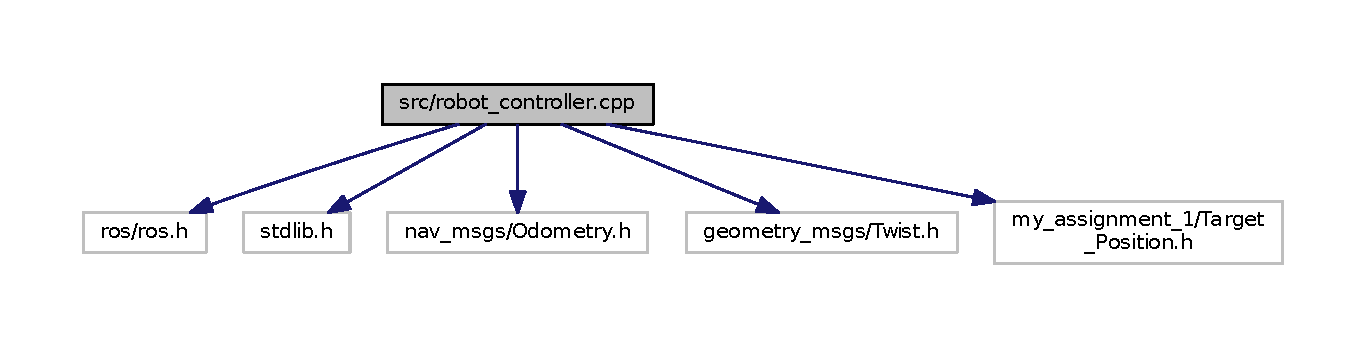
\includegraphics[width=350pt]{robot__controller_8cpp__incl}
\end{center}
\end{figure}
\subsection*{Macros}
\begin{DoxyCompactItemize}
\item 
\#define \hyperlink{robot__controller_8cpp_aa816ab3cd347f9fb8805f6296052c9c3}{alpha}~5
\end{DoxyCompactItemize}
\subsection*{Functions}
\begin{DoxyCompactItemize}
\item 
void \hyperlink{robot__controller_8cpp_aab6e381bffc34921244a29ec0538ba64}{position\+Callback} (const nav\+\_\+msgs\+::\+Odometry\+::\+Const\+Ptr \&msg)
\item 
int \hyperlink{robot__controller_8cpp_a3c04138a5bfe5d72780bb7e82a18e627}{main} (int argc, char $\ast$$\ast$argv)
\end{DoxyCompactItemize}
\subsection*{Variables}
\begin{DoxyCompactItemize}
\item 
ros\+::\+Publisher \hyperlink{robot__controller_8cpp_a350594df3e8f6948c8462edfd41ce086}{pub}
\item 
ros\+::\+Service\+Client \hyperlink{robot__controller_8cpp_a17bcd065930a8a7f9f194078d9977268}{client}
\item 
my\+\_\+assignment\+\_\+1\+::\+Target\+\_\+\+Position \hyperlink{robot__controller_8cpp_a46f6d779704275ca356cb52ef56b10a9}{target\+\_\+pos}
\item 
geometry\+\_\+msgs\+::\+Twist \hyperlink{robot__controller_8cpp_af113e9b4ca3af68972dfd3df47898c83}{vel}
\end{DoxyCompactItemize}


\subsection{Macro Definition Documentation}
\index{robot\+\_\+controller.\+cpp@{robot\+\_\+controller.\+cpp}!alpha@{alpha}}
\index{alpha@{alpha}!robot\+\_\+controller.\+cpp@{robot\+\_\+controller.\+cpp}}
\subsubsection[{\texorpdfstring{alpha}{alpha}}]{\setlength{\rightskip}{0pt plus 5cm}\#define alpha~5}\hypertarget{robot__controller_8cpp_aa816ab3cd347f9fb8805f6296052c9c3}{}\label{robot__controller_8cpp_aa816ab3cd347f9fb8805f6296052c9c3}
Define the constant to set the linear velocity proportional to the distance between the robot and the target 

\subsection{Function Documentation}
\index{robot\+\_\+controller.\+cpp@{robot\+\_\+controller.\+cpp}!main@{main}}
\index{main@{main}!robot\+\_\+controller.\+cpp@{robot\+\_\+controller.\+cpp}}
\subsubsection[{\texorpdfstring{main(int argc, char $\ast$$\ast$argv)}{main(int argc, char **argv)}}]{\setlength{\rightskip}{0pt plus 5cm}int main (
\begin{DoxyParamCaption}
\item[{int}]{argc, }
\item[{char $\ast$$\ast$}]{argv}
\end{DoxyParamCaption}
)}\hypertarget{robot__controller_8cpp_a3c04138a5bfe5d72780bb7e82a18e627}{}\label{robot__controller_8cpp_a3c04138a5bfe5d72780bb7e82a18e627}
M\+A\+IN F\+U\+N\+C\+T\+I\+ON

/\+Parameters\+: int argc, char $\ast$$\ast$argv are mandatory for cpp files

/\+Comments about the code\+:

ros\+::init--$>$initialisation of the node robot\+\_\+controller

ros\+::\+Node\+Handle n --$>$ set-\/up node\+Handle

pub=n.\+advertise$<$geometry\+\_\+msgs\+::\+Twist$>$ --$>$ declare publisher and specify the topic

ros\+::\+Subscriber sub=n.\+subscribe(\char`\"{}/odom\char`\"{},1000,position\+Callback) --$>$ define subscriber and specify the function called

client = n.\+service\+Client$<$my\+\_\+assignment\+\_\+1\+::\+Target\+\_\+\+Position$>$ --$>$ declare client and specify service type

client.\+call(target\+\_\+pos) --$>$ call manually the first time the service to generate the first random target

ros\+::spin()--$>$ blocks the main thread from exiting until R\+OS invokes a shutdown (for example Ctrl+C) \index{robot\+\_\+controller.\+cpp@{robot\+\_\+controller.\+cpp}!position\+Callback@{position\+Callback}}
\index{position\+Callback@{position\+Callback}!robot\+\_\+controller.\+cpp@{robot\+\_\+controller.\+cpp}}
\subsubsection[{\texorpdfstring{position\+Callback(const nav\+\_\+msgs\+::\+Odometry\+::\+Const\+Ptr \&msg)}{positionCallback(const nav_msgs::Odometry::ConstPtr &msg)}}]{\setlength{\rightskip}{0pt plus 5cm}void position\+Callback (
\begin{DoxyParamCaption}
\item[{const nav\+\_\+msgs\+::\+Odometry\+::\+Const\+Ptr \&}]{msg}
\end{DoxyParamCaption}
)}\hypertarget{robot__controller_8cpp_aab6e381bffc34921244a29ec0538ba64}{}\label{robot__controller_8cpp_aab6e381bffc34921244a29ec0538ba64}
/\+Function position\+Call\+Back called when subscriber receives the position

/-\/\+Parameter\+:

msg\+: declared as constant pointer of topic Odom (to establish the position of the robot)

/\+The funcion receive the position of the robot\+:

-\/\+If the robot has reached the target spawn new random target

-\/\+Else set linear velocity to reach the raget 

\subsection{Variable Documentation}
\index{robot\+\_\+controller.\+cpp@{robot\+\_\+controller.\+cpp}!client@{client}}
\index{client@{client}!robot\+\_\+controller.\+cpp@{robot\+\_\+controller.\+cpp}}
\subsubsection[{\texorpdfstring{client}{client}}]{\setlength{\rightskip}{0pt plus 5cm}ros\+::\+Service\+Client client}\hypertarget{robot__controller_8cpp_a17bcd065930a8a7f9f194078d9977268}{}\label{robot__controller_8cpp_a17bcd065930a8a7f9f194078d9977268}
Define Client that will call custom service to spawn random target \index{robot\+\_\+controller.\+cpp@{robot\+\_\+controller.\+cpp}!pub@{pub}}
\index{pub@{pub}!robot\+\_\+controller.\+cpp@{robot\+\_\+controller.\+cpp}}
\subsubsection[{\texorpdfstring{pub}{pub}}]{\setlength{\rightskip}{0pt plus 5cm}ros\+::\+Publisher pub}\hypertarget{robot__controller_8cpp_a350594df3e8f6948c8462edfd41ce086}{}\label{robot__controller_8cpp_a350594df3e8f6948c8462edfd41ce086}
Define Publisher that will publish velocity of robot on topic /cmd\+\_\+vel \index{robot\+\_\+controller.\+cpp@{robot\+\_\+controller.\+cpp}!target\+\_\+pos@{target\+\_\+pos}}
\index{target\+\_\+pos@{target\+\_\+pos}!robot\+\_\+controller.\+cpp@{robot\+\_\+controller.\+cpp}}
\subsubsection[{\texorpdfstring{target\+\_\+pos}{target_pos}}]{\setlength{\rightskip}{0pt plus 5cm}my\+\_\+assignment\+\_\+1\+::\+Target\+\_\+\+Position target\+\_\+pos}\hypertarget{robot__controller_8cpp_a46f6d779704275ca356cb52ef56b10a9}{}\label{robot__controller_8cpp_a46f6d779704275ca356cb52ef56b10a9}
Define as global an instance of service Target\+\_\+\+Position \index{robot\+\_\+controller.\+cpp@{robot\+\_\+controller.\+cpp}!vel@{vel}}
\index{vel@{vel}!robot\+\_\+controller.\+cpp@{robot\+\_\+controller.\+cpp}}
\subsubsection[{\texorpdfstring{vel}{vel}}]{\setlength{\rightskip}{0pt plus 5cm}geometry\+\_\+msgs\+::\+Twist vel}\hypertarget{robot__controller_8cpp_af113e9b4ca3af68972dfd3df47898c83}{}\label{robot__controller_8cpp_af113e9b4ca3af68972dfd3df47898c83}
Define as global an instance of the topic /cmd\+\_\+vel 
%--- End generated contents ---

% Index
\backmatter
\newpage
\phantomsection
\clearemptydoublepage
\addcontentsline{toc}{chapter}{Index}
\printindex

\end{document}
